\documentclass{article}
\usepackage[margin=0.8in]{geometry}
\usepackage{graphicx}
\usepackage{booktabs}
\usepackage{caption}
\usepackage{float}
\usepackage{subcaption}
\usepackage{amsmath}
\usepackage{amssymb}
\usepackage{hyperref}

\title{Demand Estimation Report}
\author{Airlines Merger Simulation}
% Giselle Labrador-Badia for Karam Kang and JF Houde
% University of Wisconsin-Madison
\date{\today}

\begin{document}

\maketitle

% \section{Introduction} % old when one nest 
% This report presents the results of the demand estimation analysis conducted as part of the Airlines Merger Simulation project. The tables and figures included here summarize the key findings.

% The model specification follows a logit and nested-logit framework, where consumer utility is modeled as:
% \begin{itemize}
%     \item \textbf{Logit Model:} $\ln(s_{jt}) - \ln(s_{0t}) = \alpha p_{jt} + x_{jt} \beta + \xi_t + \xi_{jt} + \epsilon_{ijt}$
%     \item \textbf{Nested-Logit Model:} $\ln(s_{jt}) - \ln(s_{0t}) = \alpha p_{jt} + x_{jt} \beta + \sigma \ln(s_{jt|g}) + \xi_t + \xi_{jt} + \epsilon_{ijt}$
% \end{itemize}
% where:
% \begin{itemize}
%     \item $p_{jt}$ is the average fare (price).
%     \item $x_{jt}$ includes regressors such as share nonstop, average distance, squared distance, and log(1 + number of fringe carriers).
%     \item $\nu_t$ and $\xi_{jt}$ are fixed effects for origin-destination and product-level unobservables.
%     \item $s_{jt|g}$ is the share of product $j$ in group $g$.
%     \item $\sigma$ captures the nesting parameter in the nested-logit model.
%     \item Instruments ($z^D_{jt}$) include average rival presence, average number of markets served by rivals, and the number of rival carriers.
% \end{itemize}

\section{Introduction}
This report presents the results of the demand estimation analysis conducted as part of the Airlines Merger Simulation project. The tables and figures included here summarize the key findings.

We estimate logit and two-level nested-logit demand. In our application, the \emph{top (group) level} partitions alternatives into \textbf{Outside} vs.\ \textbf{Inside} the air-travel market (the outside option is no trip / other modes). Within the \textbf{Inside} group, the \emph{subgroup level} partitions products into \textbf{Legacy} vs.\ \textbf{Low-Cost Carrier (LCC)}.

\section{Model and Nesting Structure}
Let $t$ index markets (e.g., OD-quarter). Products $j$ belong to a subgroup $h\in\{ \text{Legacy},\text{Non-Legacy}\}$ (or \text{LCC}) nested inside a group $g\in\{\text{Outside (not flying)},\text{Inside carrier}\}$; by convention the outside good $j=0$ belongs to $g=\text{Outside}$.

\subsection*{Utility (two-level nested logit)}
For consumer $i$ in market $t$,
\begin{align}
u_{ijt}
&= \delta_{jt} \;+\; (1-\sigma_1)\,\varepsilon_{ijt} \;+\; (\sigma_1-\sigma_2)\,\zeta_{iht} \;+\; \sigma_2\,\eta_{igt}, 
\qquad 0 \le \sigma_2 \le \sigma_1 < 1, \label{eq:util-2lvl}\\
\delta_{jt}
&= \mathbf{x}_{jt}'\beta \;+\; \alpha\,p_{jt} \;+\; \mu_t \;+\; \xi_{jt}. \label{eq:delta-mean}
\end{align}
Here $\varepsilon_{ijt},\zeta_{iht},\eta_{igt}$ are independent Type I EV shocks generating correlation within subgroups ($h$) and groups ($g$). We follow the \textbf{“\,+$\alpha p$\,”} convention in \eqref{eq:delta-mean}; economically, $\alpha<0$ is expected.

Define the scale parameters $\lambda_1 \equiv 1-\sigma_1$ (within-subgroup scale) and $\lambda_2 \equiv 1-\sigma_2$ (within-group scale), with $0<\lambda_2\le\lambda_1\le 1$.

% \subsection*{Choice probabilities}
% Let
% \[
% D_{ht} \equiv \sum_{k\in h} \exp\!\big(\delta_{kt}/\lambda_1\big), 
% \qquad 
% C_{gt} \equiv \sum_{r\in \mathcal{H}_g} D_{rt}^{\,\lambda_1/\lambda_2},
% \qquad 
% T_t \equiv \sum_{m\in\{\text{Outside},\text{Inside}\}} C_{mt}^{\,\lambda_2}.
% \]
% Then the conditional and unconditional shares are
% \begin{align}
% s_{j|h,t} &= \frac{\exp(\delta_{jt}/\lambda_1)}{D_{ht}}, 
% & s_{h|g,t} &= \frac{D_{ht}^{\,\lambda_1/\lambda_2}}{C_{gt}},
% & s_{gt} &= \frac{C_{gt}^{\,\lambda_2}}{T_t}, \\
% s_{jt} &= s_{j|h,t}\, s_{h|g,t}\, s_{gt},
% & s_{0t} &= \frac{1}{T_t}\quad (\text{outside good}). \label{eq:shares-2lvl}
% \end{align}

\subsection*{Estimating equation (two-level)}
Using the standard nested-logit inversion,
\begin{align}
\boxed{~
\log s_{jt} - \log s_{0t}
\;=\;
\mathbf{x}_{jt}'\beta \;+\; \alpha\,p_{jt}
\;+\; \sigma_2\,\log s_{j|h,t}
\;+\; \sigma_1\,\log s_{h|g,t}
\;+\; \mu_t \;+\; \xi_{jt}.
~}
\label{eq:estim-2lvl}
\end{align}
In the airline application: \\
- \emph{Group $g$}: \(\{\text{Outside},\text{Inside}\}\) (inside vs.\ outside). \\
- \emph{Subgroups $h$ within $g=\text{Inside}$}: \(\{\text{Legacy}, \text{Non-Legacy}\}\) (or \text{LCC}). \\
- For $g=\text{Outside}$, the outside good forms a degenerate subgroup.

\subsection*{Special cases}
\begin{itemize}
\item \textbf{One-level nested logit} (collapse the subgroup level): set $\sigma_1=0$ (so $\lambda_1=1$). Then
\[
\log s_{jt} - \log s_{0t}
\;=\;
\mathbf{x}_{jt}'\beta \;+\; \alpha\,p_{jt}
\;+\; \sigma_2\,\log s_{j|h,t}
\;+\; \mu_t \;+\; \xi_{jt},
\]
where now $h$ is the single (within-inside) nest (e.g., carrier-based).
\item \textbf{Multinomial logit} (no within-group correlation): set $\sigma_1=\sigma_2=0$.
\end{itemize}

\subsection*{Regressors and instruments}
We take $p_{jt}$ as average fare and $\mathbf{x}_{jt}$ to include share nonstop, (thousand-mile) distance and its square, and $\log(1+\text{rival carriers})$. We use standard rival-based shifters as instruments for $p_{jt}$ (and, if needed, for the nesting terms): average rivals' number of markets served, average rivals' route distance, and the number of rival carriers in the market-time cell.

\section{DB1B Data \& Cleaning Summary}

\begin{itemize}
  \item \textbf{Source:} DOT DB1B ``Market'' files (10\% ticket survey). Auxiliaries: city--market lookup (vacation flag), airport metadata (T\_MASTER\_CORD), airport--year populations, slot-controlled airports, carrier--airport hub table, and annual CPI index (2008{=}100; \texttt{cpi\_index.csv}).
  \item \textbf{Coverage:} Years 2005--2019; quarters 1--4; CONUS only (U.S. excluding PR, VI, TT, HI, AK), filtered via T\_MASTER\_CORD.
  \item \textbf{Market definition:} City-pair O--D level using \texttt{origincitymarketid} and \texttt{destcitymarketid}; time unit is a calendar quarter.
  \item \textbf{Product definition:} O--D--\texttt{tkcarrier}--quarter. Monopoly O--D--quarter cells dropped (require $\ge 2$ carriers).
  \item \textbf{Core filters:}
  \begin{itemize}
    \item No interline tickets: \texttt{tkcarrierchange == 0}.
    \item Real fare bounds: keep if real market fare $\in[25, 2500]$ USD, where real fare \texttt{mktfare\_real} is \texttt{mktfare} deflated using annual CPI (2008{=}100).
    \item Demand size screen at O--D--quarter: keep if total passengers $\ge 20 \times 365 / (4 \times 0.10) \approx 183$ in DB1B (i.e., at least 20 pax/day in the full universe, adjusted for the 10\% sample).
  \end{itemize}
\item \textbf{Other variables:} CONUS filter and airport names/cities from T\_MASTER\_CORD (origin/destination); slot-controlled airport indicators at origin and destination; destination ``vacation'' flag from city lookup; airport--year populations for origin and destination (nonpositive values set to missing); carrier--airport hub indicators (wide $\to$ long reshape).
  \item \textbf{Aggregation (passenger-weighted) to O--D--carrier--quarter:}
  \begin{itemize}
    \item Average distance, nonstop miles, and fare; share of nonstop; extra miles $=$ distance $-$ nonstop miles.
    \item Carrier presence at origin (origin--carrier passenger share), \# destinations from the origin, and \# markets served.
    \item Rival statistics at the O--D--quarter: average rival presence, \# markets, \# destinations, and average rival distance.
  \end{itemize}
  \item \textbf{Carriers:} Flags for carrier types (e.g., major, low-cost, legacy ) created in \texttt{carrier\_flags.do}; carrier code is \texttt{tkcarrier} (IATA 2-letter).
  \item \textbf{Output:} Final panel collapsed to O--D--carrier--quarter, with string IDs for market (\texttt{origin-destination}) and time (\texttt{year-quarter}); written to \texttt{data/processed/combined/airline\_data.csv}.
\end{itemize}

\subsection*{Variable Summary Statistics}
Lower level refers to lower nest define as \textit{legacy vs. non-legacy carriers} in the table below.

% \begin{table}[htbp]\centering
\def\sym#1{\ifmmode^{#1}\else\(^{#1}\)\fi}
\caption{Summary statistics: variables used in demand estimation}
\begin{tabular}{l*{1}{ccccccc}}
\toprule
                    &\multicolumn{7}{c}{}                                                                      \\
                    &        mean&          sd&         min&         p25&         p50&         p75&         max\\
\midrule
Market share        &       0.001&       0.006&      0.0000&      0.0001&       0.000&       0.001&       0.473\\
Outside share       &       0.992&       0.016&      0.3365&      0.9910&       0.996&       0.998&       1.000\\
Inside share sum    &       0.008&       0.016&      0.0002&      0.0024&       0.004&       0.009&       0.664\\
Nest share          &       0.008&       0.016&      0.0002&      0.0024&       0.004&       0.009&       0.664\\
Number of rival carriers&       5.477&       2.274&      1.0000&      4.0000&       5.000&       7.000&      22.000\\
Number of destinations served&      51.458&      31.554&      1.0000&     27.0000&      47.000&      75.000&     137.000\\
Average fare (dollars)&     226.831&      93.858&     25.0000&    172.4141&     212.830&     260.995&    2489.196\\
Share nonstop flights &       0.195&       0.355&      0.0000&      0.0000&       0.000&       0.143&       1.000\\
Average Distance (000s miles)&       1.491&       0.856&      0.0670&      0.8752&       1.298&       1.995&      10.345\\
Average Distance sqr (000s miles)&       2.958&       3.700&      0.0045&      0.7659&       1.686&       3.980&     107.019\\
Log(1 + fringe carriers)&       0.408&       0.469&      0.0000&      0.0000&       0.000&       0.693&       2.565\\
\midrule
Observations        &     1371742&            &            &            &            &            &            \\
\bottomrule
\end{tabular}
\end{table}

\begin{table}[htbp]\centering
\def\sym#1{\ifmmode^{#1}\else\(^{#1}\)\fi}
\caption{Summary statistics: variables used in demand estimation}
\begin{tabular}{l*{1}{ccccccc}}
\toprule
                    &\multicolumn{7}{c}{}                                                                      \\
                    &        mean&          sd&         min&         p25&         p50&         p75&         max\\
\midrule
Market share        &       0.001&       0.006&      0.0000&      0.0001&       0.000&       0.001&       0.473\\
Outside share       &       0.992&       0.016&      0.3365&      0.9908&       0.996&       0.998&       1.000\\
Inside share sum    &       0.008&       0.016&      0.0002&      0.0024&       0.004&       0.009&       0.664\\
Nest share (Upper level)&       0.008&       0.016&      0.0002&      0.0024&       0.004&       0.009&       0.664\\
Nest share (Lower level)&       0.005&       0.011&      0.0000&      0.0014&       0.003&       0.005&       0.607\\
Number of rival carriers&       5.235&       2.250&      1.0000&      4.0000&       5.000&       7.000&      22.000\\
Number of destinations served&    3583.900&    1461.539&      1.0000&   3038.0000&    4067.000&    4661.000&    5751.000\\
Average fare (dollars)&     224.884&      92.992&     25.0000&    171.7022&     212.650&     260.195&    2492.016\\
Share nonstop flights &       0.202&       0.362&      0.0000&      0.0000&       0.000&       0.167&       1.000\\
Average Distance (000s miles)&       1.494&       0.860&      0.0670&      0.8738&       1.297&       1.998&      10.345\\
Average Distance sqr (000s miles)&       2.971&       3.733&      0.0045&      0.7635&       1.683&       3.992&     107.019\\
Log(1 + fringe carriers)&       0.350&       0.455&      0.0000&      0.0000&       0.000&       0.693&       2.565\\
Average distance to rival markets&    1493.539&     830.698&     67.0000&    905.1562&    1287.021&    1982.586&    5996.580\\
Average number of rival destinations&      52.183&      26.142&      1.0000&     33.0000&      51.000&      70.000&     153.000\\
Number of rival carriers&       5.235&       2.250&      1.0000&      4.0000&       5.000&       7.000&      22.000\\
Number of rival carriers lower nest&       2.969&       1.601&      0.0000&      2.0000&       3.000&       4.000&      15.000\\
\midrule
Observations        &     1636916&            &            &            &            &            &            \\
\bottomrule
\end{tabular}
\end{table}


\pagebreak
\section{Demand Estimation Results}

Column (1) presents the results of the logit model without instruments,
while column (2) shows the logit model results with price instruments. 
Column (3) shows the nested-logit model without instruments, and 
column (4) presents the nested-logit model with instruments for both prices and nest shares.  The nests are defined as inside goods (carriers that are not the outside good) and outside good.
All columns include fixed effects for origin-destination markets. Robust standard errors are reported in parentheses below the coefficients.


%The coefficients are interpreted as elasticities, with standard errors clustered at the market level.

First, we present the basic demand estimation results. Column (1) presents the results of the logit model without instruments, while column (2) shows the logit model results with price instruments. Column (3) shows the nested-logit model without instruments, and column (4) presents the nested-logit model with one level  and instruments for both prices and nest shares.

\begin{table}[htbp]\centering
\def\sym#1{\ifmmode^{#1}\else\(^{#1}\)\fi}
\caption{Demand Estimates (Logit and Nested-Logit)}
\begin{tabular}{l*{4}{c}}
\toprule
                    &\multicolumn{1}{c}{(1)}&\multicolumn{1}{c}{(2)}&\multicolumn{1}{c}{(3)}&\multicolumn{1}{c}{(4)}\\
                    &\multicolumn{1}{c}{$\ln s_{jt}/s_{0t}$}&\multicolumn{1}{c}{$\ln s_{jt}/s_{0t}$}&\multicolumn{1}{c}{$\ln s_{jt}/s_{0t}$}&\multicolumn{1}{c}{$\ln s_{jt}/s_{0t}$}\\
\midrule
Average fare (dollars)&     -0.0017\sym{***}&      0.0102\sym{***}&     -0.0005\sym{***}&     -0.0019\sym{***}\\
                    &    (0.0000)         &    (0.0002)         &    (0.0000)         &    (0.0001)         \\
\addlinespace
Share nonstop flights &      1.9504\sym{***}&      2.0237\sym{***}&      0.1189\sym{***}&      0.3048\sym{***}\\
                    &    (0.0047)         &    (0.0057)         &    (0.0009)         &    (0.0032)         \\
\addlinespace
Average Distance (000s miles)&     -4.1437\sym{***}&     -4.5780\sym{***}&     -0.0469\sym{***}&     -0.4330\sym{***}\\
                    &    (0.0139)         &    (0.0209)         &    (0.0024)         &    (0.0091)         \\
\addlinespace
Average Distance sqr (000s miles)&      0.2762\sym{***}&      0.2153\sym{***}&      0.0043\sym{***}&      0.0398\sym{***}\\
                    &    (0.0033)         &    (0.0049)         &    (0.0005)         &    (0.0012)         \\
\addlinespace
Log(1 + fringe carriers)&     -0.5032\sym{***}&     -0.4860\sym{***}&      0.0243\sym{***}&     -0.0335\sym{***}\\
                    &    (0.0033)         &    (0.0041)         &    (0.0005)         &    (0.0010)         \\
\addlinespace
$\ln s_{jt|g}$      &                     &                     &      0.9776\sym{***}&      0.8740\sym{***}\\
                    &                     &                     &    (0.0002)         &    (0.0014)         \\
\midrule
Observations        &     1636916         &     1636916         &     1636916         &     1636916         \\
Adjusted \(R^{2}\)  &       0.503         &       0.192         &       0.983         &       0.972         \\
F-statistic (IV)    &                     &   5853.3607         &                     &   1575.4110         \\
\bottomrule
\end{tabular}
\end{table}
 

\pagebreak
\subsection{Full model, two-level nesting as legacy vs. non-legacy carriers}


Below, we present the full model results in cluding two levels of nesting and instruments for both prices and nest shares. The first column shows only one level of nesting (inside vs.\ outside), while the second column shows two levels of nesting (inside vs.\ outside, and legacy vs.\ within inside). All columns include fixed effects for origin-destination markets. Robust standard errors are reported in parentheses below the coefficients.

The instruments used are average rival distance, average number of markets served by rivals, the number of rival carriers and the number of rival carriers for the nest definition in the market. 

\begin{table}[htbp]\centering
\def\sym#1{\ifmmode^{#1}\else\(^{#1}\)\fi}
\caption{Demand Estimates (Logit and Nested-Logit)}
\begin{tabular}{l*{2}{c}}
\toprule
                    &\multicolumn{1}{c}{(1)}&\multicolumn{1}{c}{(2)}\\
                    &\multicolumn{1}{c}{$\ln s_{jt}/s_{0t}$}&\multicolumn{1}{c}{$\ln s_{jt}/s_{0t}$}\\
\midrule
Average fare (dollars)&     -0.0019\sym{***}&     -0.0021\sym{***}\\
                    &    (0.0001)         &    (0.0001)         \\
\addlinespace
Share nonstop flights &      0.3048\sym{***}&      0.2986\sym{***}\\
                    &    (0.0032)         &    (0.0050)         \\
\addlinespace
Average Distance (000s miles)&     -0.4330\sym{***}&     -0.4182\sym{***}\\
                    &    (0.0091)         &    (0.0135)         \\
\addlinespace
Average Distance sqr (000s miles)&      0.0398\sym{***}&      0.0398\sym{***}\\
                    &    (0.0012)         &    (0.0013)         \\
\addlinespace
Log(1 + fringe carriers)&     -0.0335\sym{***}&     -0.0322\sym{***}\\
                    &    (0.0010)         &    (0.0013)         \\
\addlinespace
$\ln s_{jt|g}$      &      0.8740\sym{***}&                     \\
                    &    (0.0014)         &                     \\
\addlinespace
$\ln s_{ht|g}$      &                     &      0.8866\sym{***}\\
                    &                     &    (0.0047)         \\
\addlinespace
$\ln s_{jt|h}$      &                     &      0.8753\sym{***}\\
                    &                     &    (0.0019)         \\
\midrule
Observations        &     1636916         &     1636916         \\
Adjusted \(R^{2}\)  &       0.972         &       0.972         \\
F-statistic (IV)    &   1575.4110         &    361.5578         \\
\bottomrule
\end{tabular}
\end{table}

\pagebreak
\subsection{Full model, two-level nesting as low-cost vs. non low-cost carriers}
Now I show results where the lower (second) nest is low-cost vs. non low-cost carriers.

\begin{table}[htbp]\centering
\def\sym#1{\ifmmode^{#1}\else\(^{#1}\)\fi}
\caption{Demand Estimates (Logit and Nested-Logit)}
\begin{tabular}{l*{2}{c}}
\toprule
                    &\multicolumn{1}{c}{(1)}&\multicolumn{1}{c}{(2)}\\
                    &\multicolumn{1}{c}{$\ln s_{jt}/s_{0t}$}&\multicolumn{1}{c}{$\ln s_{jt}/s_{0t}$}\\
\midrule
Average fare (dollars)&     -0.0019\sym{***}&     -0.0025\sym{***}\\
                    &    (0.0001)         &    (0.0001)         \\
\addlinespace
Share nonstop flights &      0.3048\sym{***}&      0.2799\sym{***}\\
                    &    (0.0032)         &    (0.0049)         \\
\addlinespace
Average Distance (000s miles)&     -0.4330\sym{***}&     -0.3651\sym{***}\\
                    &    (0.0091)         &    (0.0139)         \\
\addlinespace
Average Distance sqr (000s miles)&      0.0398\sym{***}&      0.0389\sym{***}\\
                    &    (0.0012)         &    (0.0014)         \\
\addlinespace
Log(1 + fringe carriers)&     -0.0335\sym{***}&     -0.0311\sym{***}\\
                    &    (0.0010)         &    (0.0011)         \\
\addlinespace
$\ln s_{jt|g}$      &      0.8740\sym{***}&                     \\
                    &    (0.0014)         &                     \\
\addlinespace
$\ln s_{ht|g}$      &                     &      0.9074\sym{***}\\
                    &                     &    (0.0043)         \\
\addlinespace
$\ln s_{jt|h}$      &                     &      0.8832\sym{***}\\
                    &                     &    (0.0020)         \\
\midrule
Observations        &     1636916         &     1636916         \\
Adjusted \(R^{2}\)  &       0.972         &       0.970         \\
F-statistic (IV)    &   1575.4110         &    396.5416         \\
\bottomrule
\end{tabular}
\end{table}


\pagebreak
\section{Elasticities}

These are observation level elasticities calculated using the parameters from the two-level nested logit model with legacy vs. non-legacy carriers as the second level nest and instruments for both prices and nest shares.

\begin{table}[htbp]\centering
\def\sym#1{\ifmmode^{#1}\else\(^{#1}\)\fi}
\caption{Elasticities: Own-price (Logit and Nested-Logit)}
\begin{tabular}{l*{1}{cccccccc}}
\toprule
                    &\multicolumn{8}{c}{}                                                                                   \\
                    &       count&        mean&          sd&         min&         p25&         p50&         p75&         max\\
\midrule
Logit Elasticity OLS&     1636916&      -0.386&       0.160&      -4.283&      -0.447&      -0.365&      -0.295&      -0.043\\
Nested-Logit Elasticity (1 Level)&     1636916&      -2.534&       1.640&     -38.207&      -3.282&      -2.460&      -1.509&      -0.048\\
Nested-Logit Elasticity (2 Levels)&     1636916&      -3.400&       1.758&     -45.444&      -4.074&      -3.205&      -2.428&      -0.085\\
\midrule
Observations        &     1636916&            &            &            &            &            &            &            \\
\bottomrule
\end{tabular}
\end{table}


When low cost vs. non low-cost carriers is used as the second level nest, the elasticities are as follows (third row).
\begin{table}[htbp]\centering
\def\sym#1{\ifmmode^{#1}\else\(^{#1}\)\fi}
\caption{Elasticities: Own-price (Logit and Nested-Logit)}
\begin{tabular}{l*{1}{cccccccc}}
\toprule
                    &\multicolumn{8}{c}{}                                                                                   \\
                    &       count&        mean&          sd&         min&         p25&         p50&         p75&         max\\
\midrule
Logit Elasticity OLS&     1636916&      -0.386&       0.160&      -4.283&      -0.447&      -0.365&      -0.295&      -0.043\\
Nested-Logit Elasticity (1 Level)&     1636916&      -2.580&       1.645&     -38.210&      -3.325&      -2.510&      -1.586&      -0.051\\
Nested-Logit Elasticity (2 Levels)&     1636916&      -4.869&       2.596&     -66.267&      -5.891&      -4.576&      -3.405&      -0.103\\
\midrule
Observations        &     1636916&            &            &            &            &            &            &            \\
\bottomrule
\end{tabular}
\end{table}


\begin{figure}[htbp]
    \centering
    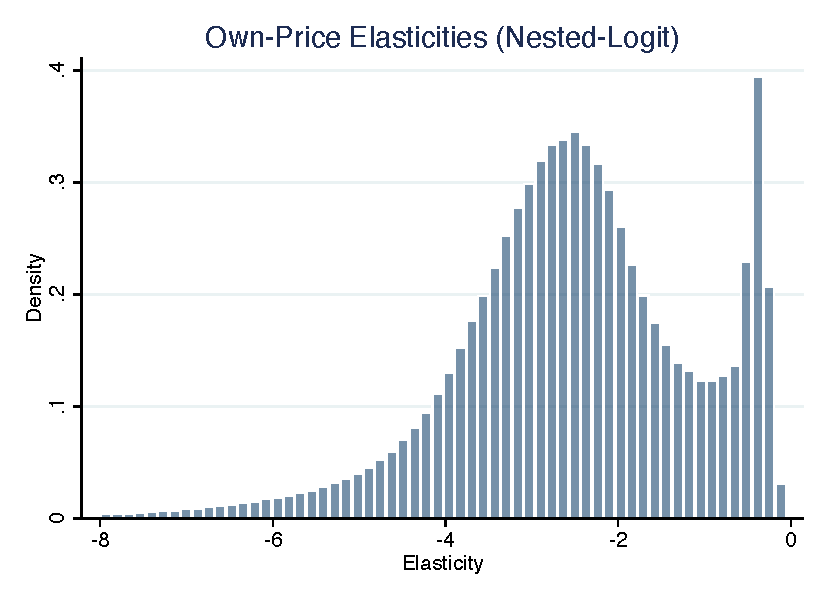
\includegraphics[width=0.7\textwidth]{../src/output/elasticity_logit_histogram_nests_lv1.pdf}
    \caption{Histogram of Elasticities, one-level nest}
\end{figure}

\begin{figure}[htbp]
    \centering
    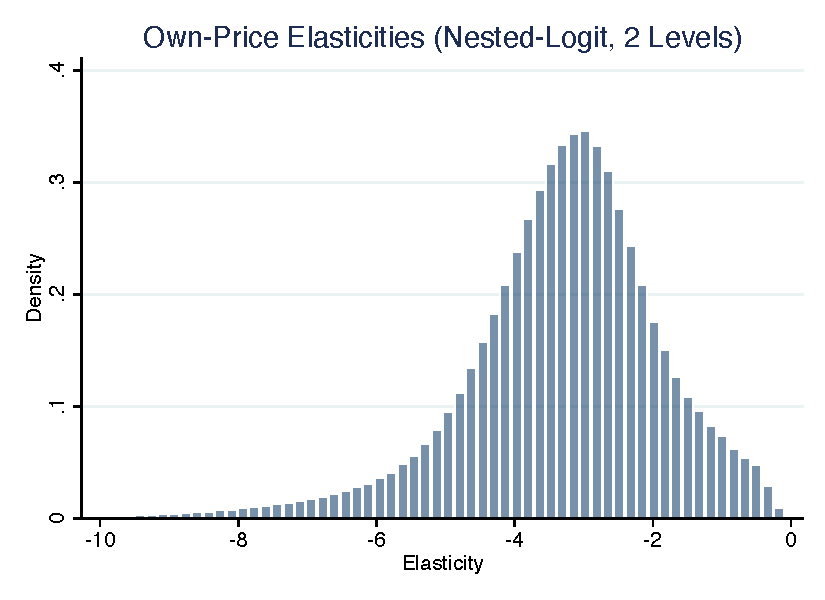
\includegraphics[width=0.7\textwidth]{../src/output/elasticity_logit_histogram_nests_lv2_legacy.pdf}
    \caption{Histogram of Elasticities, two-level nest (legacy vs. non-legacy, inside vs. outside)}
\end{figure}

\begin{figure}[htbp]
    \centering
    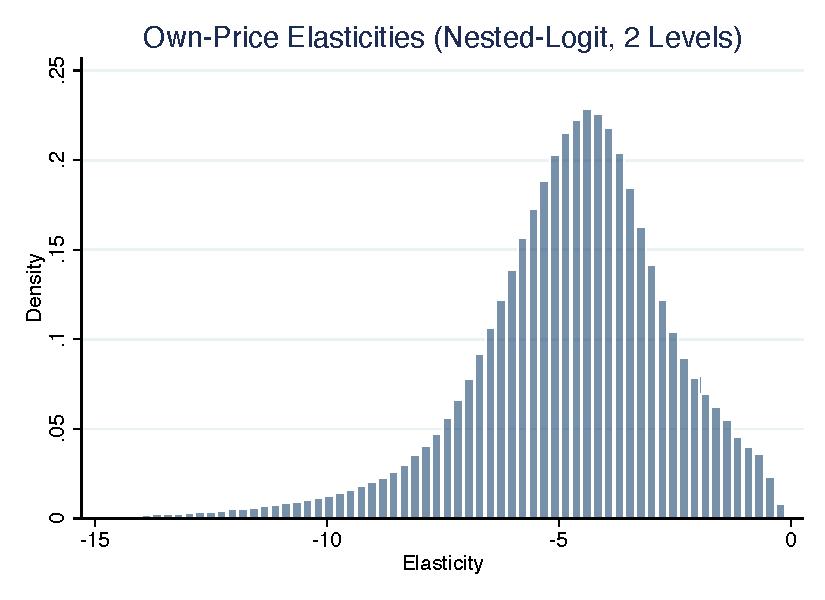
\includegraphics[width=0.7\textwidth]{../src/output/elasticity_logit_histogram_nests_lv2_lcc.pdf}
    \caption{Histogram of Elasticities, two-level nest (low-cost vs. non low-cost, inside vs. outside)}
\end{figure}
\pagebreak
\section{Appendix: First Stage Results}
\begin{table}[htbp]
    \caption{First Stage Results for Fare}
    \centering
{
\def\sym#1{\ifmmode^{#1}\else\(^{#1}\)\fi}
\begin{tabular}{l*{1}{c}}
\toprule
                    &\multicolumn{1}{c}{(1)}\\
                    &\multicolumn{1}{c}{Average fare (dollars)}\\
\midrule
Average distance to rival markets&      0.0359\sym{***}\\
                    &    (0.0008)         \\
\addlinespace
Average number of rival destinations&     -0.8452\sym{***}\\
                    &    (0.0088)         \\
\addlinespace
Number of rival carriers&    -10.9626\sym{***}\\
                    &    (0.0668)         \\
\addlinespace
Number of rival carriers lower nest&      7.8044\sym{***}\\
                    &    (0.0433)         \\
\addlinespace
Share nonstop flights &     -1.9907\sym{***}\\
                    &    (0.3057)         \\
\addlinespace
Average Distance (000s miles)&     44.5059\sym{***}\\
                    &    (1.8443)         \\
\addlinespace
Average Distance sqr (000s miles)&      4.5607\sym{***}\\
                    &    (0.4781)         \\
\addlinespace
Log(1 + fringe carriers)&      3.0140\sym{***}\\
                    &    (0.2175)         \\
\midrule
Observations        &     1636916         \\
\bottomrule
\multicolumn{2}{l}{\footnotesize Standard errors in parentheses}\\
\multicolumn{2}{l}{\footnotesize \sym{*} \(p<0.10\), \sym{**} \(p<0.05\), \sym{***} \(p<0.01\)}\\
\end{tabular}
}

\end{table}

% Below, are the first stage for the first level nest share variable.
\begin{table}[htbp]
    \caption{First Stage Results for Legacy First Level Nest Share Variable}
    \centering
    {
\def\sym#1{\ifmmode^{#1}\else\(^{#1}\)\fi}
\begin{tabular}{l*{1}{c}}
\toprule
                    &\multicolumn{1}{c}{(1)}\\
                    &\multicolumn{1}{c}{$\ln s_{ht|g}$}\\
\midrule
Average distance to rival markets&      0.0002\sym{***}\\
                    &    (0.0000)         \\
\addlinespace
Average number of rival destinations&     -0.0030\sym{***}\\
                    &    (0.0001)         \\
\addlinespace
Number of rival carriers&     -0.2373\sym{***}\\
                    &    (0.0007)         \\
\addlinespace
Number of rival carriers lower nest&      0.3606\sym{***}\\
                    &    (0.0007)         \\
\addlinespace
Share nonstop flights &      0.4507\sym{***}\\
                    &    (0.0022)         \\
\addlinespace
Average Distance (000s miles)&     -0.3959\sym{***}\\
                    &    (0.0069)         \\
\addlinespace
Average Distance sqr (000s miles)&      0.0440\sym{***}\\
                    &    (0.0015)         \\
\addlinespace
Log(1 + fringe carriers)&      0.0634\sym{***}\\
                    &    (0.0019)         \\
\midrule
Observations        &     1636916         \\
\bottomrule
\multicolumn{2}{l}{\footnotesize Standard errors in parentheses}\\
\multicolumn{2}{l}{\footnotesize \sym{*} \(p<0.10\), \sym{**} \(p<0.05\), \sym{***} \(p<0.01\)}\\
\end{tabular}
}

\end{table}

\pagebreak
Below are the first stage for the second level nest share variable for legacy nests and low-cost nests.
\begin{table}[htbp]
    \caption{First Stage Results for Legacy Nest Share Variable (Second Level)}
    \centering
    {
\def\sym#1{\ifmmode^{#1}\else\(^{#1}\)\fi}
\begin{tabular}{l*{1}{c}}
\toprule
                    &\multicolumn{1}{c}{(1)}\\
                    &\multicolumn{1}{c}{$\ln s_{jt|h}$}\\
\midrule
Average distance to rival markets&      0.0014\sym{***}\\
                    &    (0.0000)         \\
\addlinespace
Average number of rival destinations&     -0.0167\sym{***}\\
                    &    (0.0002)         \\
\addlinespace
Number of rival carriers&     -0.0430\sym{***}\\
                    &    (0.0012)         \\
\addlinespace
Number of rival carriers lower nest&     -0.3756\sym{***}\\
                    &    (0.0009)         \\
\addlinespace
Share nonstop flights &      1.4283\sym{***}\\
                    &    (0.0045)         \\
\addlinespace
Average Distance (000s miles)&     -3.4366\sym{***}\\
                    &    (0.0126)         \\
\addlinespace
Average Distance sqr (000s miles)&      0.1948\sym{***}\\
                    &    (0.0027)         \\
\addlinespace
Log(1 + fringe carriers)&     -0.1177\sym{***}\\
                    &    (0.0039)         \\
\midrule
Observations        &     1636916         \\
\bottomrule
\multicolumn{2}{l}{\footnotesize Standard errors in parentheses}\\
\multicolumn{2}{l}{\footnotesize \sym{*} \(p<0.10\), \sym{**} \(p<0.05\), \sym{***} \(p<0.01\)}\\
\end{tabular}
}

\end{table}

\begin{table}[htbp]
    \caption{First Stage Results for Low-Cost Nest Share Variable (Second Level)}
    \centering
    {
\def\sym#1{\ifmmode^{#1}\else\(^{#1}\)\fi}
\begin{tabular}{l*{1}{c}}
\toprule
                    &\multicolumn{1}{c}{(1)}\\
                    &\multicolumn{1}{c}{$\ln s_{jt|h}$}\\
\midrule
Average distance to rival markets&      0.0015\sym{***}\\
                    &    (0.0000)         \\
\addlinespace
Average number of rival destinations&     -0.0153\sym{***}\\
                    &    (0.0002)         \\
\addlinespace
Number of rival carriers&     -0.0293\sym{***}\\
                    &    (0.0012)         \\
\addlinespace
Number of rival carriers lower nest&     -0.3489\sym{***}\\
                    &    (0.0009)         \\
\addlinespace
Share nonstop flights &      1.5496\sym{***}\\
                    &    (0.0046)         \\
\addlinespace
Average Distance (000s miles)&     -3.4022\sym{***}\\
                    &    (0.0136)         \\
\addlinespace
Average Distance sqr (000s miles)&      0.1871\sym{***}\\
                    &    (0.0031)         \\
\addlinespace
Log(1 + fringe carriers)&     -0.0541\sym{***}\\
                    &    (0.0039)         \\
\midrule
Observations        &     1636916         \\
\bottomrule
\multicolumn{2}{l}{\footnotesize Standard errors in parentheses}\\
\multicolumn{2}{l}{\footnotesize \sym{*} \(p<0.10\), \sym{**} \(p<0.05\), \sym{***} \(p<0.01\)}\\
\end{tabular}
}

\end{table}


\end{document}
